\documentclass[11pt]{article}
\usepackage[a4paper,margin=2.4cm]{geometry}
\usepackage{amsmath,amssymb,amsthm}
\usepackage{graphicx}
\usepackage[font=small,labelfont=bf]{caption}
\usepackage{subcaption}
\usepackage[colorlinks=true,allcolors=blue]{hyperref}
\usepackage{microtype}

\newtheorem{theorem}{Theorem}
\newtheorem{corollary}{Corollary}
\newcommand{\Iop}{\hat{I}}
\newcommand{\tr}{\operatorname{Tr}}
\newcommand{\KL}{D_{\mathrm{KL}}}

\title{\bfseries Fixation of a time-reversal-odd observable by decoherence:\\
record distinguishability as the local arrow of time\\
in an exactly solvable model}
\author{Mostfa Lejri\\[2pt]
\small Independent Researcher}
\date{\small Extended version: \today}

\begin{document}
\maketitle

\begin{abstract}
\noindent
The microscopic laws of physics are invariant under time reversal, yet every observer records a fixed arrow of time. We study how decoherence fixes the orientation of a time-reversal-odd observable in an exactly solvable model: a three-site chiral ring, whose degenerate current-carrying doublet forms a T-odd pointer basis, coupled to a bath of recording qubits. The model admits closed forms for all bipartite entropies, and its two-branch structure reduces trajectory statistics to classical inference. We prove that the unconditional stochastic entropy production vanishes identically (the arrow is spontaneously broken, existing only relative to a branch) and that the branch-relative entropy production equals exactly the accumulated Kullback--Leibler distinguishability $D(t)$ of the environmental records. Numerically, chirality fixation locks to decoherence ($t_P/t_S$ saturating at $0.956\pm0.003$ for bath sizes $N\ge64$), while Darwinian redundancy lags by a factor of four: the observable fixes before it becomes objective. Branch polarization collapses onto a universal function of $D$ across protocols and couplings, with no detectable hysteresis under record degradation. Measuring the records converts the revocable arrow into a ratchet. Classicalization of records, not decoherence alone, makes the local arrow permanent.
\end{abstract}

\tableofcontents

\section{Introduction}

Irreversibility is not written in the dynamical laws. Newtonian, quantum and relativistic dynamics are time-reversal symmetric, and the standard resolutions of this tension (the thermodynamic arrow from special initial conditions \cite{Albert2000}, the psychological arrow from the physics of memory \cite{Mlodinow2014}, the decoherent arrow from environmental monitoring \cite{Zeh2007,Zurek2003,Guff2025}) share a common intuition: the arrow of time is carried by \emph{records}.

Two research programmes have, independently, made the record concept quantitative. Quantum Darwinism \cite{Zurek2009,Riedel2012,Zurek2022} identifies the objective, classical properties of a system with those whose information has proliferated redundantly into the environment: a property is objective when many observers can read it independently from small, disjoint environmental fragments, and the redundancy $R_\delta$ measures how many such fragments exist. Throughout, objectivity is quantified by mutual-information redundancy in the original sense of quantum Darwinism \cite{Ollivier2004,Zurek2009}; in our exactly solvable two-branch model the strong refinements of objectivity (spectrum broadcast structure, strong quantum Darwinism \cite{Korbicz2021,Le2019}) essentially coincide with it, since the conditional environment states become orthogonal products, so the distinction carries no weight here. Stochastic thermodynamics \cite{Maes2003,Callens2004,Landi2021}, meanwhile, identifies the irreversibility of a process with the log-ratio of the probabilities of a trajectory and of its time reverse: entropy production is, by theorem, a measure of time-reversal breaking. These two quantifications (of objectivity and of irreversibility) have developed with essentially no contact; the discussion of Ref.~\cite{Riedel2012} explicitly lists the connection to quantum-trajectory methods as open. Recent proposals that classicality and the arrow of time co-emerge at a threshold, as an amplification-driven symmetry-breaking transition \cite{Aharonov2000}, have remained at the level of postulated order parameters.

This paper connects the two frameworks in a model simple enough to be solved exactly, and specifically constructed so that the question is sharp: its pointer observable is odd under time reversal, so that fixing it \emph{is} breaking time-reversal symmetry locally. Position or spin-$z$ pointer bases, standard in decoherence models, are T-even; a decohered position tells us nothing about temporal orientation. A \emph{current}, by contrast, reverses under T: einselection of a circulation direction is einselection of an arrow. Our results are fourfold. (i) The model (a three-site chiral ring monitored by a qubit bath) is exactly solvable, in both its baseline and record-degrading variants (Sec.~\ref{sec:model}). (ii) The unconditional stochastic entropy production vanishes identically, while the branch-relative entropy production equals the accumulated record distinguishability, exactly (Sec.~\ref{sec:arrow}, Theorems~\ref{th:zero} and \ref{th:identity}). (iii) Numerically, chirality fixation locks to decoherence while redundancy lags fourfold, and all quantities collapse onto a universal function of the record information (Sec.~\ref{sec:numerics}). (iv) With coherent, degradable records the local arrow is fully revocable, riding the universal curve in both directions; measuring the records converts it into a ratchet (Sec.~\ref{sec:variantB}). Section~\ref{sec:discussion} discusses limitations, the relation to threshold proposals, and a flux-qubit realization. Appendices collect closed forms, proofs, and numerical protocols.

\section{The model}\label{sec:model}

\subsection{A T-odd pointer doublet}

The system is a single spinless particle on a three-site ring, the minimal system with a well-defined sense of circulation. In the site basis $\{|0\rangle,|1\rangle,|2\rangle\}$ (indices mod 3, $\hbar=1$, $J=1$),
\begin{equation}
H_S = -J\sum_{j=0}^{2}\big(|j\rangle\langle j{+}1| + |j{+}1\rangle\langle j|\big),
\qquad
\Iop = iJ\sum_{j=0}^{2}\big(|j{+}1\rangle\langle j| - |j\rangle\langle j{+}1|\big).
\end{equation}
The quasimomentum states $|k\rangle = 3^{-1/2}\sum_j e^{ikj}|j\rangle$, $k\in\{0,\pm2\pi/3\}$, diagonalize both operators, with $E_k=-2J\cos k$ and $\Iop|k{=}{\pm}2\pi/3\rangle = \pm I_0\,|k{=}{\pm}2\pi/3\rangle$, $I_0=\sqrt3 J$. The two current-carrying states, henceforth $|\pm\rangle$, are degenerate ($E=+J$): a chiral doublet. Three properties, verified symbolically and numerically in the accompanying repository, structure everything below: $[H_S,\Iop]=0$ (the current is conserved, so the chiral states are \emph{exact} pointer states and the decoherence is pure); under the antiunitary $K_{\mathrm{ring}}$ (complex conjugation in the site basis) one has $K\Iop K^{-1}=-\Iop$ and $K|\pm\rangle=|\mp\rangle$ (the pointer observable is T-odd and T exchanges the branches); and the initial state
\begin{equation}
|\psi_S(0)\rangle = \tfrac{1}{\sqrt2}\big(|+\rangle+|-\rangle\big)
\end{equation}
is T-invariant up to a phase, with $\langle\Iop\rangle=0$: a state for which the local temporal orientation is genuinely undefined. The $k{=}0$ state is excluded by the initial condition and never populated. This doublet has an experimental realization: superconducting flux qubits, whose clockwise/counterclockwise persistent-current superpositions are precisely such T-odd doublets \cite{Friedman2000}. The einselection of a degenerate chiral doublet has a venerable precedent: the environmental superselection of molecular handedness that resolves Hund's paradox \cite{Harris1981,Trost2009}. The crucial difference is the discrete symmetry involved: molecular handedness is parity-odd, so its fixation breaks P and carries no information about time; the circulation doublet is T-odd, and its fixation is precisely a local breaking of time-reversal symmetry, which is what permits the co-analysis with process irreversibility below.

\subsection{Recording bath and exact solvability}

The environment is $N$ qubits coupled to the current,
\begin{equation}
H = H_S\otimes\mathbb1 + \frac{\Iop}{I_0}\otimes\sum_{n=1}^{N} g_n\,\sigma_z^{(n)}
\;\Big({+}\sum_n \omega_n\sigma_x^{(n)}\ \text{in variant B}\Big),
\label{eq:H}
\end{equation}
with couplings $g_n$ drawn uniformly from $[\bar g/2,3\bar g/2]$ and the bath initialized in $|+_x\rangle^{\otimes N}$. Because the chirality is conserved, the global state remains a sum of exactly two branch products at all times,
\begin{equation}
|\Psi(t)\rangle = \tfrac{1}{\sqrt2}\Big(|+\rangle\bigotimes_n|\phi^{(n)}_+(t)\rangle
+ |-\rangle\bigotimes_n|\phi^{(n)}_-(t)\rangle\Big),
\qquad
|\phi^{(n)}_s(t)\rangle = e^{-i(s\,g_n\sigma_z+\omega_n\sigma_x)t}|+_x\rangle.
\label{eq:branches}
\end{equation}
Every bipartite reduced state of $S\cup F$ ($F$ any bath fragment) therefore has rank $\le2$, with von Neumann entropy $S = H_2\!\big((1{+}|c|)/2\big)$, $H_2$ the binary entropy and $c$ the appropriate product of single-qubit overlaps $c_n(t)=\langle\phi^{(n)}_-|\phi^{(n)}_+\rangle$ (Appendix~\ref{app:entropies}). In the baseline ($\omega_n=0$), $c_n(t)=\cos(2g_nt)$ and the decoherence factor is $r(t)=\prod_n\cos(2g_nt)$. Brute-force state-vector evolution at $N=8$ agrees with these closed forms to $5\times10^{-14}$; the analytic engine then powers all large-$N$ results. Two remarks on the status of these idealizations. Exact degeneracy of the doublet is not fine-tuning but the statement of the problem: a splitting between $|+\rangle$ and $|-\rangle$ is a current bias, itself T-odd, so imposing it would break time-reversal symmetry in the law rather than let it break spontaneously, exactly as a ferromagnet is studied at zero external field. And the legitimate T-even perturbation, a tunneling $\Delta$ between the chiralities, places the model in the standard competition between pointer states and energy eigenstates: in the strong-monitoring regime $g\gg\Delta$ (the quantum measurement limit underlying pure-dephasing models since their inception \cite{Zurek2003}) chirality einselection survives approximately; quantifying that crossover is left for future work. Mathematically, tracing out the ring reduces the construction to the exactly solvable central-spin dephasing model that has anchored einselection studies since their origin \cite{Zurek1981,Riedel2012}; the new ingredient is not the mathematics but the symmetry: the central ``spin'' is a chiral doublet whose basis states are exchanged by time reversal, and the monitored observable is T-odd, which is what opens the co-analysis with process irreversibility.

\begin{figure}[t]
\centering
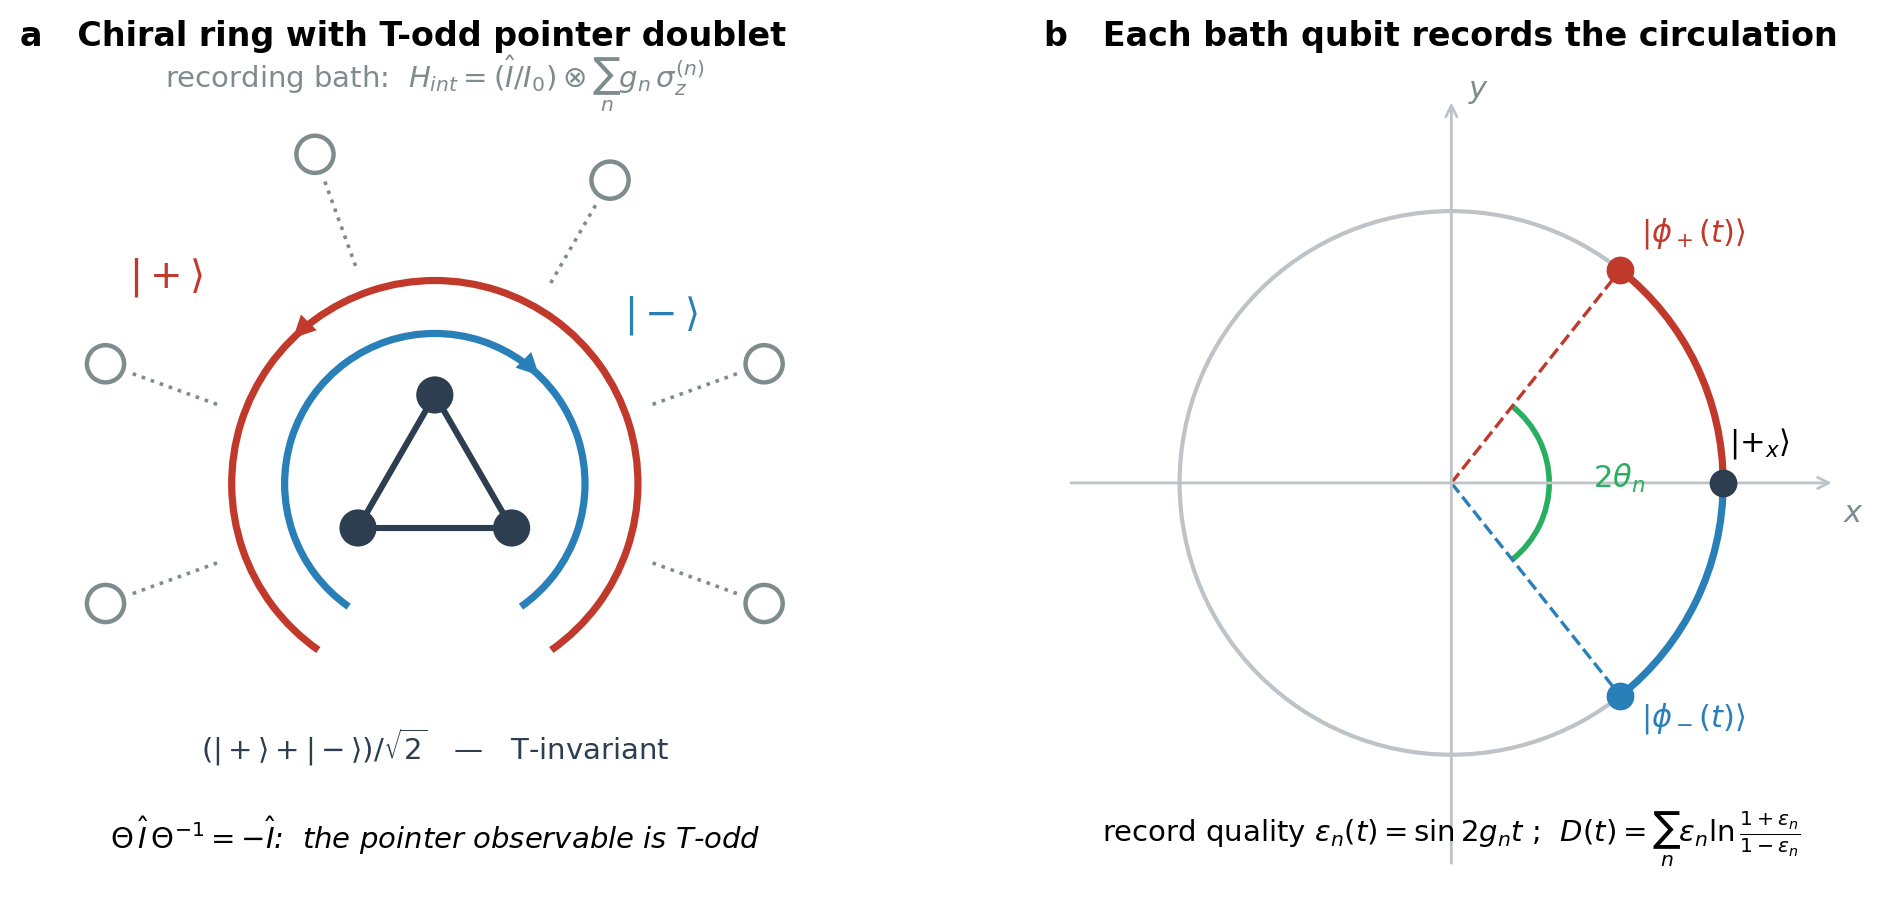
\includegraphics[width=0.92\linewidth]{fig1_schematic.png}
\caption{\textbf{The model.} \textbf{a}, Three-site chiral ring with degenerate circulation doublet $|\pm\rangle$ and recording bath. \textbf{b}, Conditional trajectories of one bath qubit on the Bloch equator; the growing angle constitutes the record, of quality $\varepsilon_n(t)=\sin 2g_nt$.}
\label{fig:model}
\end{figure}

\subsection{Trajectory protocols}

Two measurement protocols are used. In the \emph{snapshot} protocol, all bath qubits are measured at time $t$ in the $\sigma_y$ basis (which is Helstrom-optimal for discriminating the conditional states (Appendix~\ref{app:helstrom})) yielding record quality $\varepsilon_n(t)=\sin(2g_nt)$ per qubit. In the \emph{collision} protocol, qubit $n$ interacts only during $[t_{n-1},t_n]$ and is measured at $t_n$, yielding permanent records with $\varepsilon_n=\sin(2g_n\Delta t)$ and monotone dynamics free of finite-size revivals. In both, conditioning on the branch $s=\pm1$ (a hidden fair coin drawn at $t=0$) makes the outcomes independent biased bits,
\begin{equation}
P(r_n|s) = \frac{1+r_n\,s\,\varepsilon_n}{2},
\label{eq:forward}
\end{equation}
so the entire trajectory statistics reduces to classical inference on the branch. Measuring the bath never back-acts on $\rho_S$ ($\Iop$ is conserved), so the monitored and unmonitored versions share identical unconditional system dynamics: redundancy is computed on the unmonitored model, entropy production on the monitored one.

\section{The arrow is branch-relative and equals record information}\label{sec:arrow}

\subsection{Time reversal and the backward process}

The correct antiunitary for the baseline is $\Theta = K_{\mathrm{ring}}\otimes(i\sigma_yK)^{\otimes N}$: it flips both the current and $\sigma_z$, so $\Theta H\Theta^{-1}=H$; the total dynamics is microreversible, and all time asymmetry lives in states and branches, not in the law. (The naive choice $\Theta=K$ on everything makes $H_{\mathrm{int}}$ T-odd and wrecks the construction; in variant B the correct operator is instead $K_{\mathrm{ring}}\otimes(\sigma_xK)^{\otimes N}$, which flips $\sigma_z$ while preserving $\sigma_x$.) The backward process is the $\Theta$-conjugate of the forward protocol: $\Theta$-imaged preparation ($\Theta|+_x\rangle\propto|-_x\rangle$), motion-reversed evolution, and $\Theta$-imaged detectors \emph{retaining their forward labels}; the T-oddness of the recorded datum enters through the trajectory conjugation $\tilde\xi$ (reversed order, $\tilde r_n=-r_n$). Direct computation, verified to machine precision (Appendix~\ref{app:proofs}), gives
\begin{equation}
P_{\mathrm{bwd}}(\tilde r_n|s') = \frac{1-\tilde r_n\,s'\,\varepsilon_n}{2}.
\label{eq:backward}
\end{equation}

\subsection{Two exact results}

\begin{theorem}[Spontaneous breaking of the arrow]\label{th:zero}
For the symmetric initial superposition, the unconditional stochastic entropy production vanishes trajectory by trajectory:
$\sigma[\xi]=\ln P_{\mathrm{fwd}}(\xi)-\ln P_{\mathrm{bwd}}(\tilde\xi)=0$ for every record $\xi$.
\end{theorem}

\begin{proof}
$P_{\mathrm{fwd}}(\xi)=\tfrac12\sum_s\prod_n(1+r_ns\varepsilon_n)/2$ and, by Eq.~\eqref{eq:backward} with $\tilde r_n=-r_n$,
$P_{\mathrm{bwd}}(\tilde\xi)=\tfrac12\sum_{s'}\prod_n(1+r_ns'\varepsilon_n)/2$: the double sign flip $r\to-r$, $s\to-s$ restores the forward expression after summing over the symmetric branch prior.
\end{proof}

The ensemble has no arrow, exactly as a ferromagnet ensemble has no magnetization. The asymmetry is spontaneously broken and exists only relative to a branch. We stress what distinguishes this from ordinary state-level T-breaking: a ferromagnet also einselects a T-odd observable, yet fixes no arrow. The claim here rests on the exact identity between the fixation of the state and the irreversibility of the process (the same variable $D$ governs both) and on the ratchet, which ties the permanence of the orientation to the modal status of the records; neither has a magnetic analogue. We use ``spontaneously broken'' in an operational, finite-size sense, exactly as finite-size einselection selects one of two symmetry-related pointer sectors: the ensemble remains rigorously T-symmetric while every conditioned history occupies one of two T-conjugate record sectors. We claim no thermodynamic phase transition; consistently, the transition does not sharpen with $N$ in the record variable. This is not a deficiency of the model but its central structural feature, and Theorem~\ref{th:zero} doubles as an exactness test for the numerics.

For an observer \emph{within} a branch, the chirality $s$ is a fact: their memories are themselves records conditioned on $s$ \cite{Mlodinow2014}, and the operationally accessible reversal is the $\Theta$-conjugated protocol within the same branch; the observer cannot conjugate the fact $s$; $\Theta$ would map their world to the other branch. Define the branch-relative stochastic entropy production
\begin{equation}
\sigma_s[\xi] \equiv \ln P(\xi|s) - \ln P_{\mathrm{bwd}}(\tilde\xi|s)
= \sum_n \ln\frac{1+r_n s\,\varepsilon_n}{1-r_n s\,\varepsilon_n}.
\label{eq:sigma_s}
\end{equation} Throughout, entropy production is meant in this operational, stochastic-thermodynamic sense of a log-ratio of forward and backward record probabilities; what it quantifies here is informational irreversibility relative to a record-bearing observer, not energetic dissipation.

\begin{theorem}[The arrow is record information]\label{th:identity}
$\displaystyle \langle\sigma_s\rangle
= \sum_n \varepsilon_n\ln\frac{1+\varepsilon_n}{1-\varepsilon_n}
= \sum_n \KL\!\big[p(r_n|s)\,\big\|\,p(r_n|{-}s)\big] \;\equiv\; D(t) .$
\end{theorem}

\begin{proof}
Average Eq.~\eqref{eq:sigma_s} over $r_n\sim(1{+}r_ns\varepsilon_n)/2$ per record; each term gives $\varepsilon_n\ln[(1{+}\varepsilon_n)/(1{-}\varepsilon_n)]$, which is the KL divergence between the Bernoulli distributions of the two branches.
\end{proof}

\begin{corollary}[Fluctuation theorem]
$\langle e^{-\sigma_s}\rangle = 1$ exactly, per record:
$\sum_r \frac{1+r\varepsilon}{2}\cdot\frac{1-r\varepsilon}{1+r\varepsilon} = 1$.
\end{corollary}

Theorem~\ref{th:identity} is the paper's central claim in exact form: \textbf{the irreversibility of the process, as experienced within a branch, is identically the information content of the environmental records about the T-odd datum}. Irreversibility and record formation are not merely correlated in this model; under the branch-relative definition, they are the same quantity. We emphasize that the identity is not definitional: both sides have independent definitions from disjoint literatures, and the equality \emph{fails} for a T-even pointer observable, for which the branch-relative backward statistics coincides with the forward one and $\langle\sigma_s\rangle=0$ while $D$ grows. The equality encodes a physical fact specific to T-odd einselection: time reversal and branch exchange are the same operation. The alternative, $\Theta$-conjugated-branch comparison gives identically zero (Theorem~\ref{th:zero}'s conditional analogue) and carries no information: the arrow \emph{is} the branch-relativity.

\section{Numerical results}\label{sec:numerics}

\subsection{Validation and the canonical Darwinism structure}

The partial-information plots $\bar I(S{:}F_m)$ (Fig.~\ref{fig:pip}) reproduce the canonical antisymmetric shape of quantum Darwinism \cite{Riedel2012}: rapid rise to the classical plateau at $S(\rho_S)$, then the quantum jump to $2S(\rho_S)$ as the fragment approaches the full environment. The sampled entropy production tracks the closed form of Theorem~\ref{th:identity} with relative deviation decreasing as $n_{\mathrm{traj}}^{-1/2}$ down to $10^{-4}$; the integral fluctuation theorem holds to one per cent for up to ten records, beyond which the estimator variance grows exponentially, as is generic \cite{Landi2021}.

\begin{figure}[t]
\centering
\begin{subfigure}[t]{0.49\linewidth}
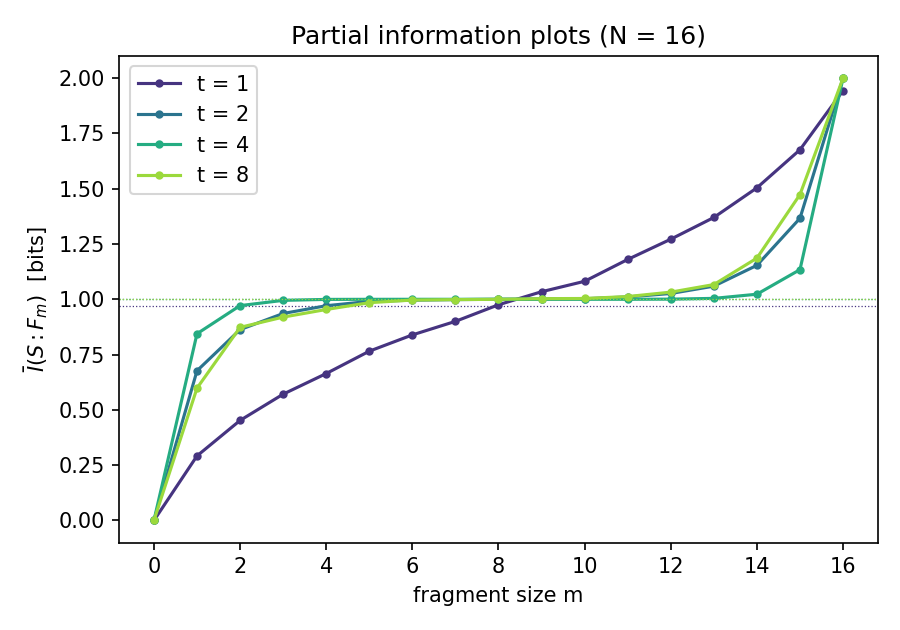
\includegraphics[width=\linewidth]{fig1_pip.png}
\caption{}
\end{subfigure}\hfill
\begin{subfigure}[t]{0.49\linewidth}

\includegraphics[width=\linewidth]{fig2_cotransition.png}
\caption{}
\end{subfigure}
\caption{\textbf{Baseline snapshot protocol ($N=16$).} \textbf{a}, Partial information plots at four times: the canonical Darwinism shape. \textbf{b}, Co-transition curves; oscillations at late times are finite-size revivals of the cosine products, removed by the collision protocol of Fig.~\ref{fig:collision}.}
\label{fig:pip}
\end{figure}

\subsection{Fixation precedes objectivity}

Figure~\ref{fig:collision} tracks four quantities through the transition in the collision protocol: the system entropy $S(\rho_S)$, the branch polarization $P=\mathbb E_\xi|2q(\xi)-1|$ (with $q$ the Bayes posterior over branches; the conditional current obeys $\langle\Iop\rangle_\xi = I_0(2q-1)$ exactly), the record distinguishability $D$, and the redundancy $R_\delta$. The hierarchy is strict. Polarization locks to decoherence: across bath sizes $N=8$ to $256$ the ratio of half-rise times is $0.953\pm0.005$ pooled over ten disorder realizations per size, with a weak finite-size drift ($0.945\pm0.003$ at $N=8$) that saturates at $0.956\pm0.003$ beyond $N\approx64$ (Fig.~\ref{fig:scaling}b); in the large-bath limit the two timescales lock at a fixed sub-unit ratio, polarization marginally leading, since the posterior concentrates as soon as any record discriminates the branches while the system's coherence requires the full overlap product to die. Redundancy lags fourfold: the chirality is \emph{fixed} long before it is \emph{objective}, consistent with the continued growth of redundancy after decoherence saturates \cite{Riedel2012}. The conditional-current distribution evolves from unimodal at zero to sharply bimodal at $\pm I_0$ (Fig.~\ref{fig:hist}): spontaneous T-symmetry breaking at branch level. All timescales scale as $N^{-1/2}$ (Fig.~\ref{fig:scaling}a) and the transition does not sharpen relative to its own width: in the record variable there is no critical threshold.

\begin{figure}[t]
\centering

\includegraphics[width=0.72\linewidth]{fig4_collision.png}
\caption{\textbf{Collision protocol ($N=120$, $\Delta t=0.6$).} Monotone co-transition: $P$ locks to $S(\rho_S)$, redundancy lags, and the sampled $\langle\sigma\rangle$ (dotted) falls exactly on the closed form $D$ of Theorem~\ref{th:identity}.}
\label{fig:collision}
\end{figure}

\begin{figure}[t]
\centering
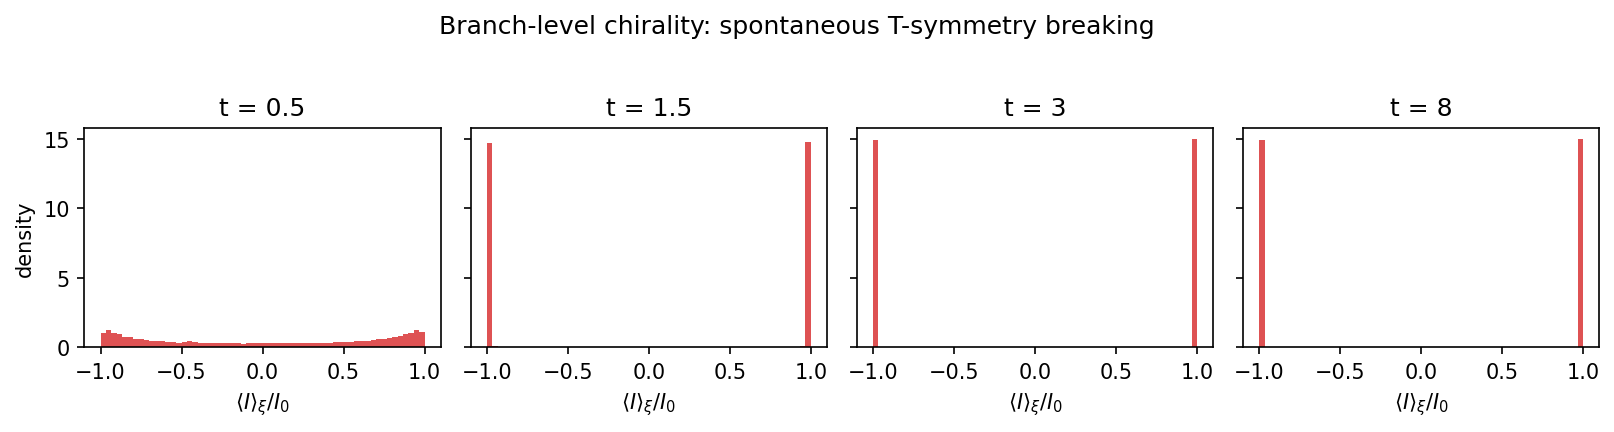
\includegraphics[width=0.9\linewidth]{fig3_histograms.png}
\caption{\textbf{Spontaneous T-symmetry breaking at branch level.} Distribution of the conditional current across sampled records: unimodal and time-symmetric before the transition, bimodal at $\pm I_0$ after.}
\label{fig:hist}
\end{figure}

\begin{figure}[t]
\centering
\begin{subfigure}[t]{0.49\linewidth}
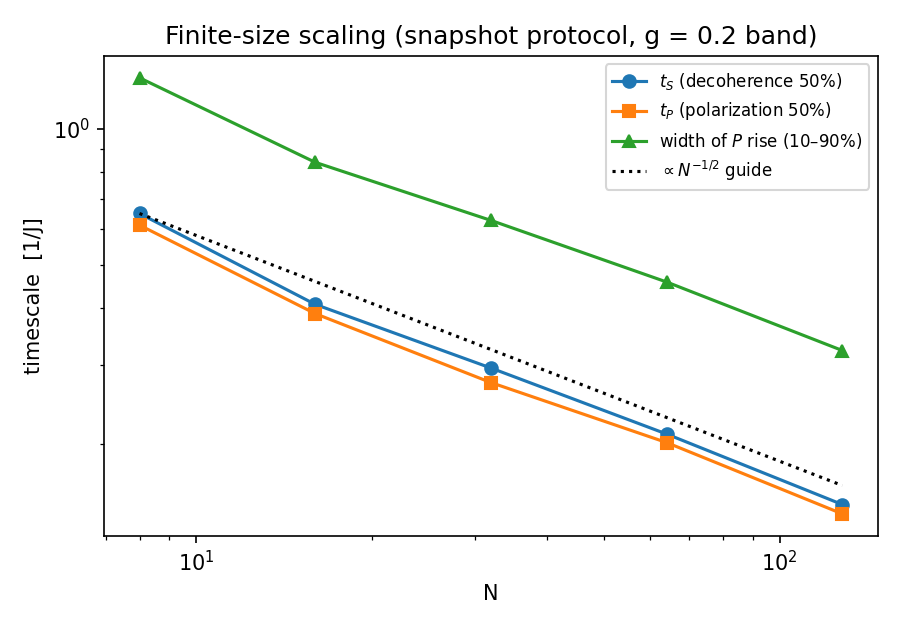
\includegraphics[width=\linewidth]{fig5_scaling.png}
\caption{}
\end{subfigure}\hfill
\begin{subfigure}[t]{0.49\linewidth}
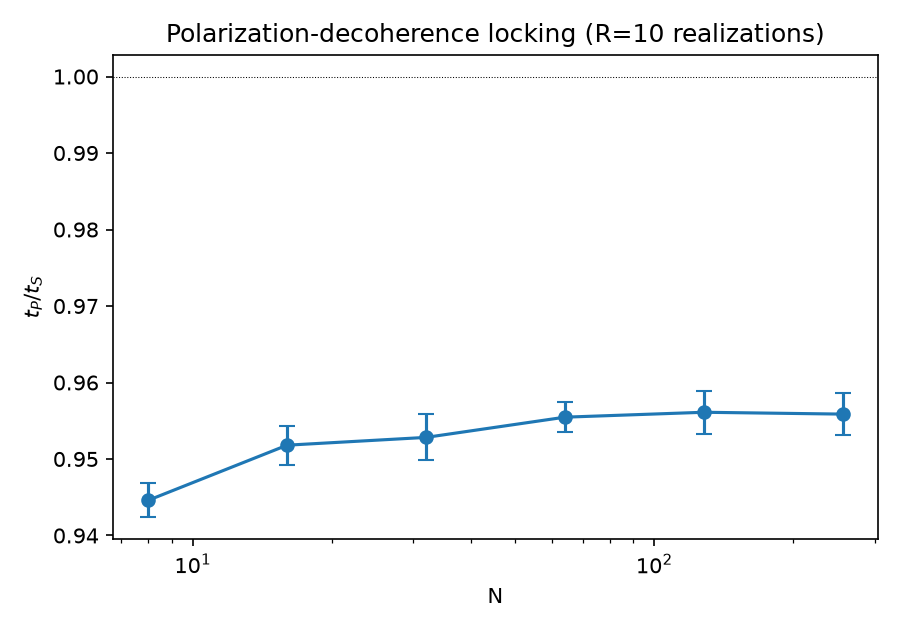
\includegraphics[width=\linewidth]{fig5b_ratio_errorbars.png}
\caption{}
\end{subfigure}
\caption{\textbf{Finite-size scaling.} \textbf{a}, All timescales $\propto N^{-1/2}$; the relative width of the transition is $N$-independent. \textbf{b}, The ratio $t_P/t_S$ over ten disorder realizations per size: weak drift saturating at $0.956\pm0.003$ beyond $N\approx64$.}
\label{fig:scaling}
\end{figure}

\subsection{Universality}

Across bath sizes, coupling strengths and both protocols, the branch polarization collapses onto a single sigmoid $P(D)$ of the accumulated distinguishability (Fig.~\ref{fig:collapse}a); explained by Theorem~\ref{th:identity}: entropy production, polarization and redundancy are all functionals of the same per-record divergences $\{\varepsilon_n\}$. The collapse is tight: root-mean-square residual $0.005$, maximum $0.024$ (bootstrap 95\% CI $[0.017,0.024]$), with the master curve estimated by a quantile-binned running median over ten disorder realizations.

\begin{figure}[t]
\centering
\begin{subfigure}[t]{0.49\linewidth}
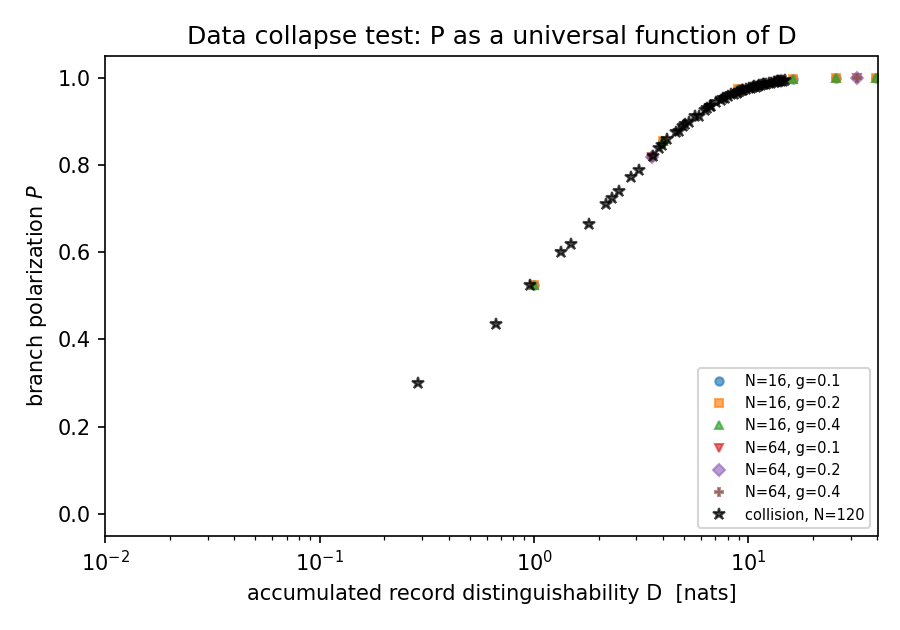
\includegraphics[width=\linewidth]{fig6_collapse.png}
\caption{}
\end{subfigure}\hfill
\begin{subfigure}[t]{0.49\linewidth}
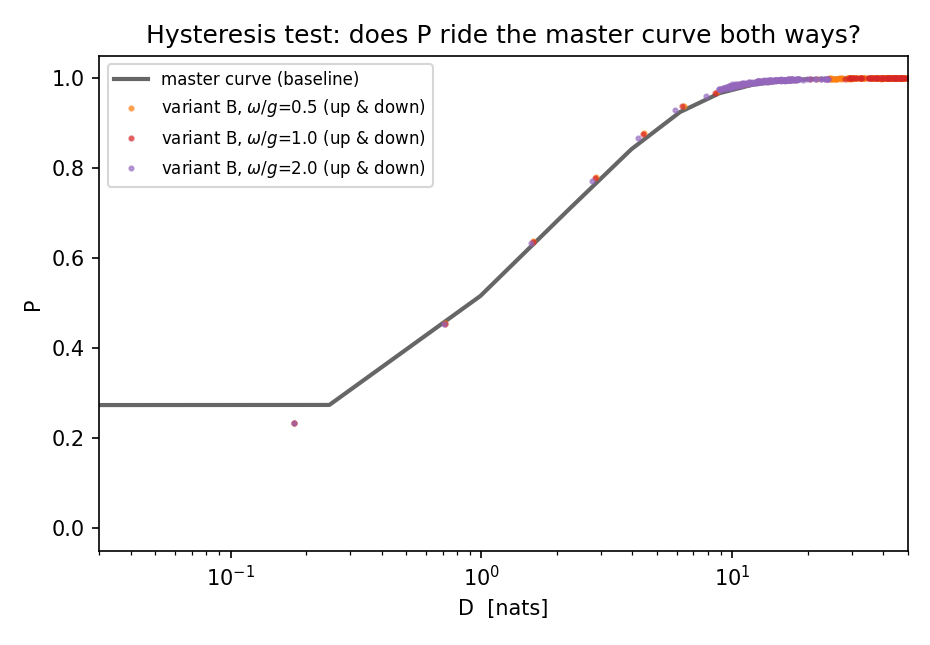
\includegraphics[width=\linewidth]{fig8_hysteresis.png}
\caption{}
\end{subfigure}
\caption{\textbf{One universal curve, ridden in both directions.} \textbf{a}, $P$ versus $D$ for six parameter sets and two protocols. \textbf{b}, With degrading and reviving records (variant B, three ratios $\omega/\bar g$), the $(D,P)$ trajectory rides the same master curve up and down; maximal residual $0.017$, decreasing with trajectory number (sampling floor).}
\label{fig:collapse}
\end{figure}

\section{Degrading records: revocability and the ratchet}\label{sec:variantB}

Adding the bath self-Hamiltonian $\sum_n\omega_n\sigma_x^{(n)}$ preserves the two-branch structure \eqref{eq:branches} (the model remains exactly solvable through conditional $2\times2$ Rabi rotations) while making the records degradable: the conditional Bloch vectors can reconverge, $|c_n(t)|$ revives, and the Helstrom record quality $\varepsilon_n(t)=\sqrt{1-|c_n(t)|^2}$ becomes non-monotone. Figure~\ref{fig:variantB} shows the resulting rise and fall of distinguishability and redundancy across three ratios $\omega/\bar g$, the degrading-record analogue of the rise and fall of redundancy under interacting environments \cite{Riedel2012}.

\begin{figure}[t]
\centering
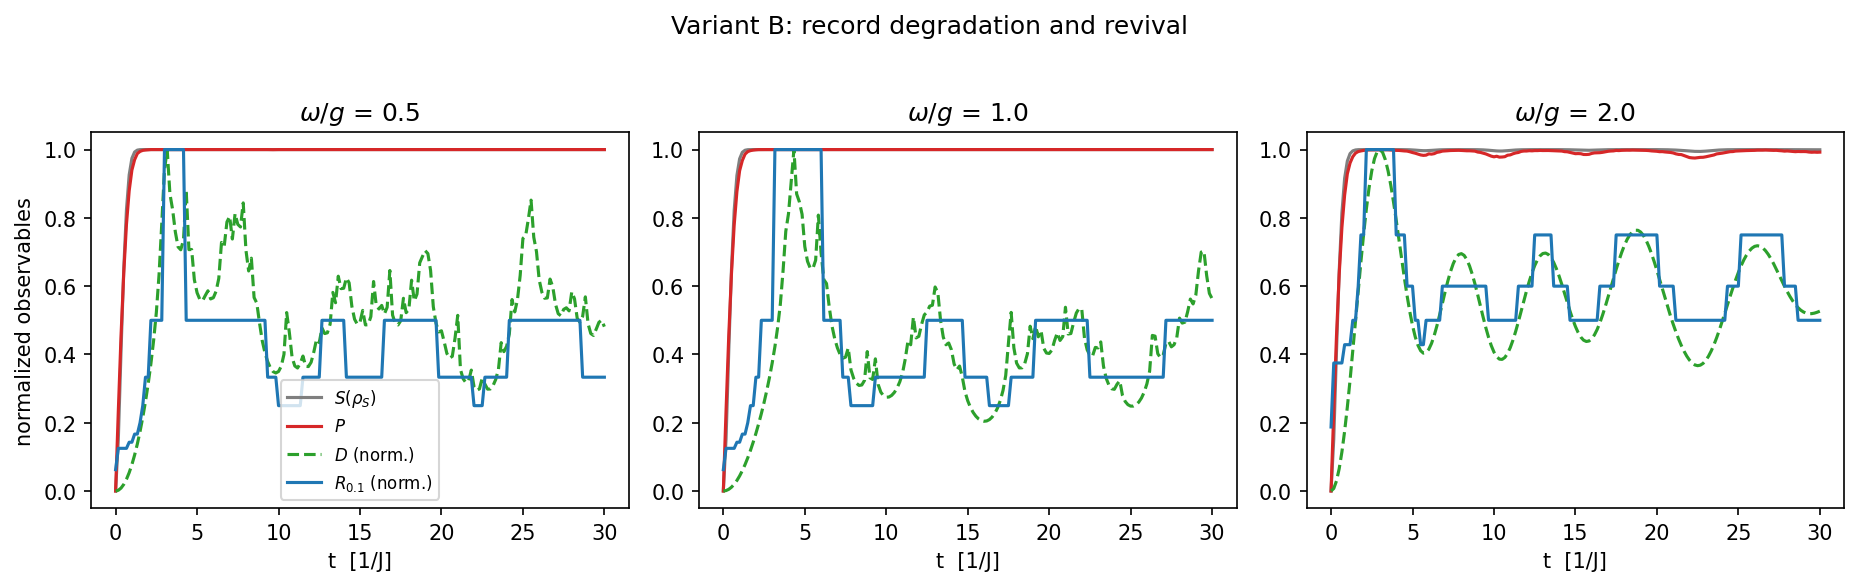
\includegraphics[width=0.98\linewidth]{fig7_variantB.png}
\caption{\textbf{Variant B: record degradation and revival} for $\omega/\bar g = 0.5, 1, 2$ ($N=16$). $D$ and $R_\delta$ oscillate as records recohere.}
\label{fig:variantB}
\end{figure}

Two results follow. First, \emph{single-scalar sufficiency under degradation}: in the snapshot protocol the polarization is by construction memoryless in the instantaneous record qualities, so retracing is structural; what is not guaranteed is that the one-dimensional summary $D$ remains sufficient as the record-quality distribution deforms. It does: as $D(t)$ falls and rises the polarization stays on the universal curve of Fig.~\ref{fig:collapse}a in both directions, with residuals bounded by $0.017$ and decreasing with trajectory number, a sampling floor (Fig.~\ref{fig:collapse}b). While the records remain quantum, the local arrow is fully revocable: when the environment recoheres, the branch orientation unfixes along exactly the path by which it fixed. Second, the \emph{ratchet}: running the identical degrading dynamics but measuring each bath qubit once (classicalizing its record) makes the polarization monotone (Fig.~\ref{fig:ratchet}). Throughout, permanent means precisely this: immune to any subsequent recoherence of the original quantum records, once those records have been classicalized. Each measured record is a click that no recoherence can undo. The contrast isolates the precise role of the quantum-to-classical transition: decoherence fixes the orientation of a T-odd observable within a branch; redundant proliferation makes it objective; only the classicalization of the records makes it \emph{permanent}. The arrow of time inherits the modal status of the records that carry it.

\begin{figure}[t]
\centering
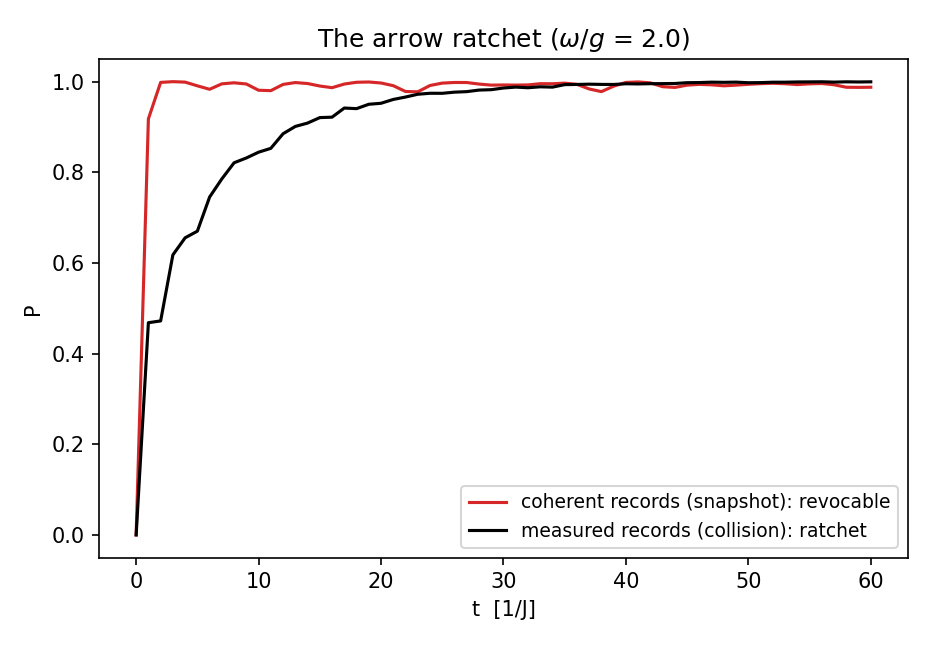
\includegraphics[width=0.62\linewidth]{fig9_ratchet.png}
\caption{\textbf{The classicalization ratchet} ($\omega/\bar g=2$). Coherent records: revocable, oscillating polarization. Measured records: monotone ratchet.}
\label{fig:ratchet}
\end{figure}

\section{Discussion}\label{sec:discussion}

Three limitations bound the claims. The ring is spatial and its T-odd observable is a current: the model demonstrates decoherence-driven local breaking of time-reversal symmetry of the \emph{state}, co-analysed with the irreversibility of the \emph{process}; it does not model the emergence of time itself and, like all emergence-of-classicality arguments, presupposes a dynamics with a locality structure. Two clarifications sharpen this boundary. The mechanism itself is generic (any T-odd observable monitored by a recording environment undergoes the same branch-level fixation, and records beget records) so a contagion of local arrows into a consistent global one is a natural conjecture; but what would propagate is the thermodynamic orientation (the direction of record accumulation), not the randomly einselected chirality, and demonstrating alignment across many systems requires a multi-system model we have not built. And the asymmetry that does propagate is inherited from the initial condition: the record-free product state of the bath is a Past Hypothesis in miniature \cite{Chen2024}, so the model derives the local arrow \emph{given} an initially record-free environment, and defers the origin of that condition to cosmology, where it belongs \cite{Halliwell1994}. Complementary channel-level notions of irreversible classicality (monotone contraction of coherence functionals relative to a fixed conjugation \cite{Gil2026}) address the approach to classicality of the map rather than the T-symmetry of the state, and are compatible with the present state-level analysis. A related objection deserves a direct answer: the model contains no heat, work, or dissipation, so one may ask whether $\sigma$ deserves the name entropy production at all. That is by design: the construction isolates the informational component of the arrow with zero energetic confound, within the measurement-inclusive framework of stochastic thermodynamics \cite{Landi2021}; adding dissipative channels would add entropy production, not replace the record term. The branch-relative definition \eqref{eq:sigma_s} is a choice. We defend it on the grounds that the alternative (conjugating the branch) is unavailable to any observer whose memories are themselves records within the branch \cite{Mlodinow2014}, and yields identically zero information. Finally, our universal sigmoid is smooth: standard decoherence plus redundancy produces no sharp threshold in the record variable. This sharpens rather than undermines the testability of proposals in which the quantum--classical transition is a genuine critical phenomenon \cite{Aharonov2000}: any observed threshold-like disappearance of interference at a critical noise or amplification level would be a departure from the exactly solvable baseline established here.

The flux-qubit realization of the chiral doublet \cite{Friedman2000} suggests that the polarization--distinguishability curve, and the ratchet contrast, are measurable with existing circuit-QED techniques: the required ingredients are a persistent-current qubit, an engineered bath of ancilla qubits coupled to the circulating current, and the choice of reading the ancillas out (ratchet) or letting them evolve (revocable arrow). More broadly, the model turns a metaphysical question (when does time acquire a direction?) into an operational one: the local arrow is fixed when, and only for as long as, the environment can tell a process from its time reverse; it becomes objective when many can tell independently; and it becomes irrevocable only when their records do.

\appendix

\section{Closed-form entropies}\label{app:entropies}
From the two-branch structure \eqref{eq:branches}, the reduced state of $S\cup F$ is supported on the orthogonal pair $|{+},E_+^F\rangle$, $|{-},E_-^F\rangle$ with off-diagonal weight $c_{\bar F}=\prod_{n\notin F}c_n$, giving eigenvalues $(1\pm|c_{\bar F}|)/2$. Hence
\begin{equation}
I(S{:}F) = H_2\!\Big(\tfrac{1+|c_Fc_{\bar F}|}{2}\Big) + H_2\!\Big(\tfrac{1+|c_F|}{2}\Big) - H_2\!\Big(\tfrac{1+|c_{\bar F}|}{2}\Big),
\end{equation}
with $c_F=\prod_{n\in F}c_n$. Redundancy $R_\delta = N/m_\delta$, with $m_\delta$ the smallest fragment size whose average mutual information reaches $(1-\delta)S(\rho_S)$; $\delta=0.1$ throughout, with sensitivity checked at $\delta\in\{0.05,0.2\}$.

\section{Proof details and verification}\label{app:proofs}
Equation~\eqref{eq:forward}: conditional on $s$, qubit $n$ ends at angle $2sg_n\tau$ from $+x$ on the equator; projection on $\sigma_y$ eigenstates gives $(1\pm\sin 2sg_n\tau)/2$. Equation~\eqref{eq:backward}: with $\Theta$-conjugated evolution (in backward-branch label $s'$: $e^{+is'g_n\tau\sigma_z}$) applied to $\Theta|+_x\rangle\propto|-_x\rangle$ and $\Theta$-imaged detectors retaining forward labels, direct computation gives $(1-\tilde r s'\varepsilon)/2$. All steps of Theorems~\ref{th:zero}--\ref{th:identity}, the labeling convention, and the identity $\langle\Iop\rangle_\xi=I_0(2q-1)$ (by exhaustive enumeration at $N=4$) are verified by an independent numerical suite in the repository; the suite caught and fixed one labeling-convention error in an earlier draft of the backward protocol, which we record here as a caution: with T-odd data, whether $\Theta$-imaged detectors keep or flip their labels is not a matter of taste but is fixed by consistency with the trajectory conjugation.

\section{Helstrom optimality and variant B}\label{app:helstrom}
In the baseline the two conditional qubit states are symmetric about the $x$ axis; the Helstrom measurement for equal priors is $\sigma_y$, with success probability $(1+\varepsilon_n)/2$, $\varepsilon_n=\sqrt{1-|c_n|^2}=|\sin 2g_nt|$. In variant B, $|\phi_s^{(n)}(t)\rangle = e^{-i(sg_n\sigma_z+\omega_n\sigma_x)t}|+_x\rangle$ is an analytic Rabi rotation; the optimal basis is time- and qubit-dependent, and $\varepsilon_n(t)=\sqrt{1-|c_n(t)|^2}$ throughout. Microreversibility in variant B holds with $\Theta=K_{\mathrm{ring}}\otimes(\sigma_xK)^{\otimes N}$.

\section{Numerical protocols}\label{app:numerics}
Statistics: errors are standard deviations over ten disorder realizations; trajectory sampling $5\times10^4$ per point ($3\times10^5$ for the hysteresis floor test); master curve by quantile-binned running median over 200 time points per realization; bootstrap (200 resamples) for the CI on the maximal residual. Redundancy: 150 fragment samples per size. Code ($\approx$700 lines, Python/NumPy) with fixed seeds at \url{https://github.com/lejrimostfa/chiral-ring}; every figure regenerates by a single command.


\section*{Acknowledgments}
This work made extensive use of Anthropic's Claude (a large language model) as a research assistant, for model design discussions, derivations, code, and manuscript drafting. Every analytic claim was verified by an independently recoded numerical suite to machine precision. This verification loop caught and corrected one convention error during development. The author reviewed all derivations and takes sole and full responsibility for the content.

\begin{thebibliography}{99}\small
\bibitem{Zeh2007} H.~D. Zeh, \emph{The Physical Basis of the Direction of Time} (Springer, 2007).
\bibitem{Zurek1981} W.~H. Zurek, Pointer basis of quantum apparatus: Into what mixture does the wave packet collapse?, \emph{Phys. Rev. D} \textbf{24}, 1516 (1981); Environment-induced superselection rules, \emph{Phys. Rev. D} \textbf{26}, 1862 (1982).
\bibitem{Zurek2003} W.~H. Zurek, \emph{Rev. Mod. Phys.} \textbf{75}, 715 (2003).
\bibitem{Ollivier2004} H.~Ollivier, D.~Poulin, W.~H. Zurek, Objective properties from subjective quantum states, \emph{Phys. Rev. Lett.} \textbf{93}, 220401 (2004).
\bibitem{Zurek2009} W.~H. Zurek, \emph{Nat. Phys.} \textbf{5}, 181 (2009).
\bibitem{Riedel2012} C.~J. Riedel, W.~H. Zurek, M.~Zwolak, \emph{New J. Phys.} \textbf{14}, 083010 (2012).
\bibitem{Zurek2022} W.~H. Zurek, \emph{Entropy} \textbf{24}, 1520 (2022).
\bibitem{Mlodinow2014} L.~Mlodinow, T.~A. Brun, \emph{Phys. Rev. E} \textbf{89}, 052102 (2014).
\bibitem{Chen2024} J.~Al-Khalili, E.~K. Chen, The decoherent arrow of time and the entanglement past hypothesis, \emph{Found. Phys.} \textbf{54}, 49 (2024).
\bibitem{Guff2025} T.~Guff, C.~U. Shastry, A.~Rocco, Emergence of opposing arrows of time in open quantum systems, \emph{Sci. Rep.} \textbf{15}, 3658 (2025).
\bibitem{Aharonov2000} D.~Aharonov, Quantum to classical phase transition in noisy quantum computers, \emph{Phys. Rev. A} \textbf{62}, 062311 (2000).
\bibitem{Albert2000} D.~Z. Albert, \emph{Time and Chance} (Harvard Univ. Press, 2000).
\bibitem{Maes2003} C.~Maes, K.~Neto\v{c}n\'y, \emph{J. Stat. Phys.} \textbf{110}, 269 (2003).
\bibitem{Callens2004} I.~Callens, W.~De Roeck, T.~Jacobs, C.~Maes, K.~Neto\v{c}n\'y, \emph{Physica D} \textbf{187}, 383 (2004).
\bibitem{Landi2021} G.~T. Landi, M.~Paternostro, \emph{Rev. Mod. Phys.} \textbf{93}, 035008 (2021).
\bibitem{Gil2026} J.~J. Gil, Intrinsic pointer basis and irreversible classicality from coherence contraction, arXiv:2604.23304 (2026).
\bibitem{Harris1981} R.~A. Harris, L.~Stodolsky, On the time dependence of optical activity, \emph{J. Chem. Phys.} \textbf{74}, 2145 (1981).
\bibitem{Trost2009} J.~Trost, K.~Hornberger, Hund's paradox and the collisional stabilization of chiral molecules, \emph{Phys. Rev. Lett.} \textbf{103}, 023202 (2009).
\bibitem{Halliwell1994} J.~J. Halliwell, J.~P\'erez-Mercader, W.~H. Zurek (eds.), \emph{Physical Origins of Time Asymmetry} (Cambridge Univ. Press, 1994).
\bibitem{Korbicz2021} J.~K. Korbicz, Roads to objectivity: quantum Darwinism, spectrum broadcast structures, and strong quantum Darwinism, \emph{Quantum} \textbf{5}, 571 (2021).
\bibitem{Le2019} T.~P. Le, A.~Olaya-Castro, Strong quantum Darwinism and strong independence are equivalent to spectrum broadcast structure, \emph{Phys. Rev. Lett.} \textbf{122}, 010403 (2019).
\bibitem{Friedman2000} J.~R. Friedman \emph{et al.}, \emph{Nature} \textbf{406}, 43 (2000).
\end{thebibliography}

\end{document}
